\section{Hyperbolic geometry}

\subsection{Normal polygons and fundamental regions}

%Vonroi diagram

\begin{figure}
\centering
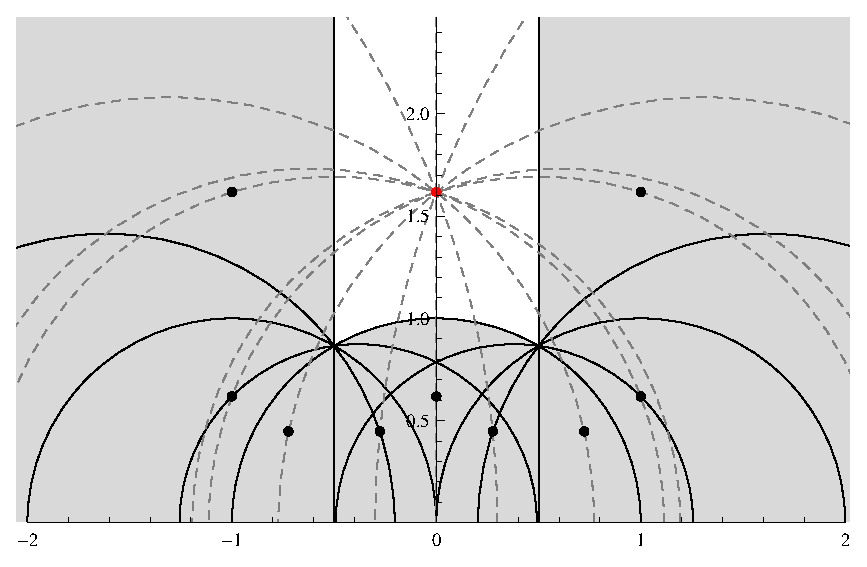
\includegraphics[width=\textwidth]{figures/normpoly-fundom-1}
\caption[The fundamental region $\FunDom$ as normal polygon]{The fundamental region $\FunDom$ can alternatively obtained by constructing the normal polygon with respect to a point $z$ on the imaginary axis with $\Im{z} > 1$. Above the point $z = \phi \ii$ (red) has been chosen, where $\phi = \frac{\sqrt{5}+1}{2}$ denotes the golden ratio.}
\label{fig_NormalPolyFunDom}
\end{figure}

\begin{figure}
\centering
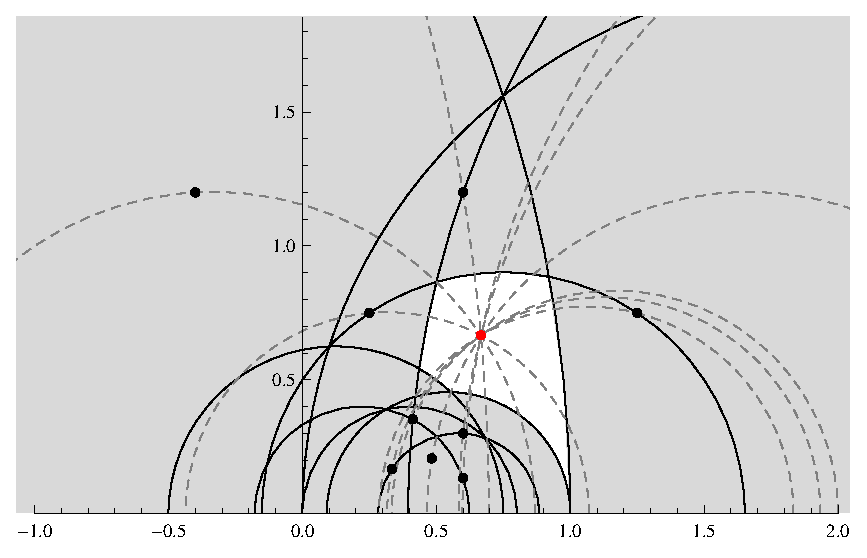
\includegraphics[width=\textwidth]{figures/normpoly-fundom-2}
\caption[An alternative fundamental region for $\PSL{\Z}$]{An alternative fundamental region for the action of $\PSL{\Z}$ on $\EU$. It is obtained by constructing the normal polygon for the point $\frac{2}{3}(1+\ii)$.}
\label{fig_AltNormalPolyFunDom}
\end{figure}

\begin{figure}
\centering
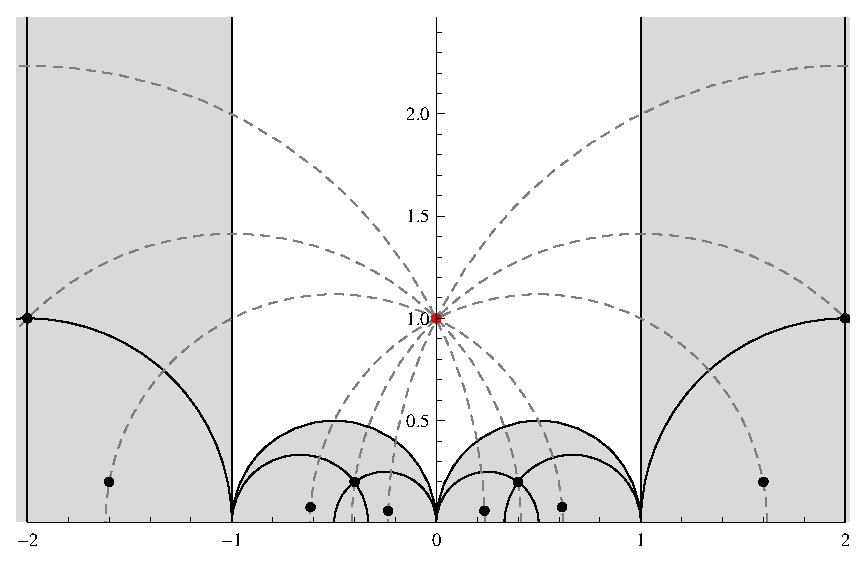
\includegraphics[width=\textwidth]{figures/normpoly-gamma2-1}
\caption[A fundamental region $\Gamma(2)$]{A fundamental region for the subgroup $\Gamma(2) \le \PSL{\Z}$. It is given by the normal polygon constructed with respect to the point $\ii$.}
\label{fig_Gamma2NormalPoly}
\end{figure}
